\documentclass[10pt,a4paper,oneside]{article}

\usepackage[swedish]{babel}
\usepackage[utf8]{inputenc}
\usepackage[T1]{fontenc}
\usepackage{graphicx}
\usepackage{color}
\usepackage{float}
\usepackage{url}



 
\title{<Dokumentets titel>}
\author{Författare}
\date{\today}

\begin{document}

\maketitle
\newpage

\section{Sammanfattning}
\newpage

\tableofcontents
\newpage

\section{Introduktion}
\newpage

\section{Bakgrund}
\newpage

\section{Metod}
\newpage

\section{Beskrivning av tjänsten}
\subsection{Vad erbjuder vi för tjänst?}
\subsection{Hur blir man medlem?}
\subsection{Vad krävs för att bli medlem?}
\subsection{Hur ska hemsidan och appen utformas?}
\subsection{Kvalitetskontroll}
\subsection{Förpackning av varor}
\subsection{Order och leverans}
\subsection{Framtida expansionsmöjligheter för tjänsten }
\newpage

\section{Koppling till energisystemet}
\newpage

\section{Canvas modellen}
\subsection{Värdeerbjudande}
\subsection{Kundsegment}
\subsection{Kanaler}
\subsection{Kundrelation}
\subsection{Intäktsström}
\subsection{Nyckelresurser}
\subsection{Nyckelaktiviteter}
\subsection{Nyckelpartners}
\subsection{Kostnadsstruktur}
\newpage

\section{Marknadsundersökning}
\newpage

\section{Ekonomisk budget}
\newpage

\section{Konkurrenter}
\newpage

\section{Analyser}
\subsection{Val av affärsmodell}
\subsection{Scenarioanalys  - yttre faktorer}
\subsection{SWOT- analys}
\newpage

\section{Diskussion}
\newpage

\section{Slutsats}
\newpage

\bibliographystyle{amsplain}
\bibliography{litterature}
\newpage

\section*{Bilagor}

\begin{figure}[H]
	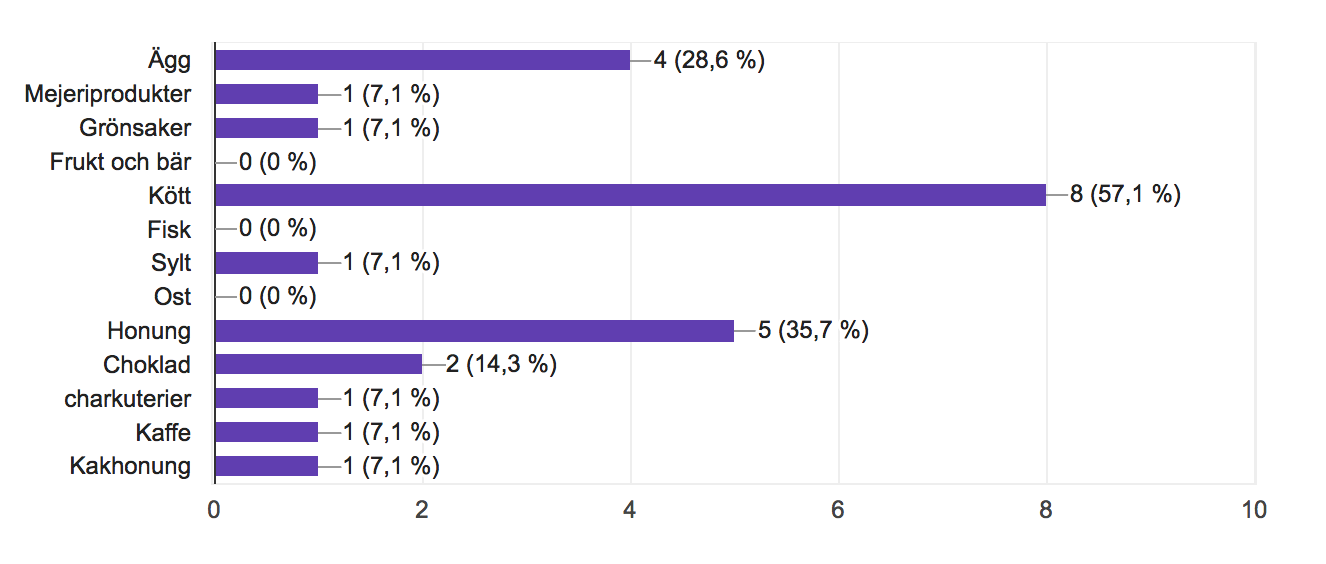
\includegraphics[scale=0.6]{1.png}
\end{figure}

\begin{figure}[H]
	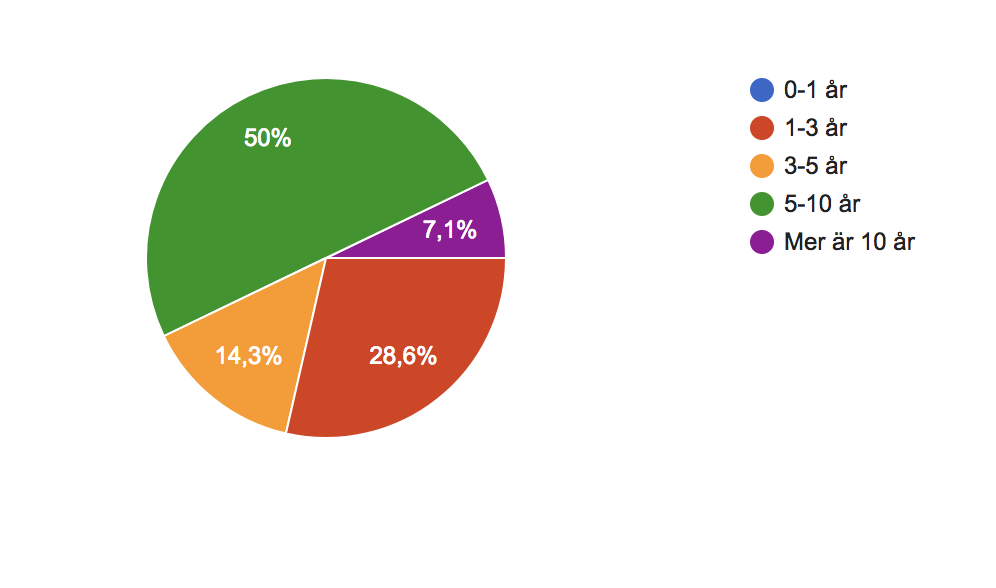
\includegraphics[scale=0.6]{2.png}
\end{figure}

\begin{figure}[H]
	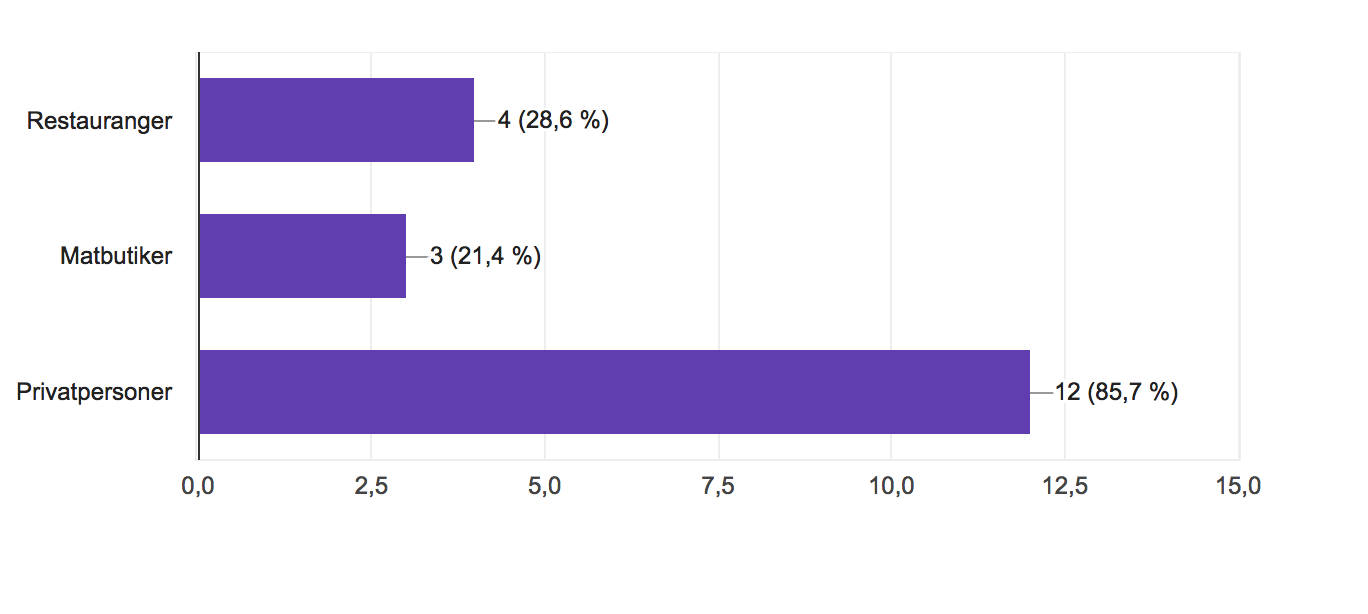
\includegraphics[scale=0.6]{3.png}
\end{figure}

\begin{figure}[H]
	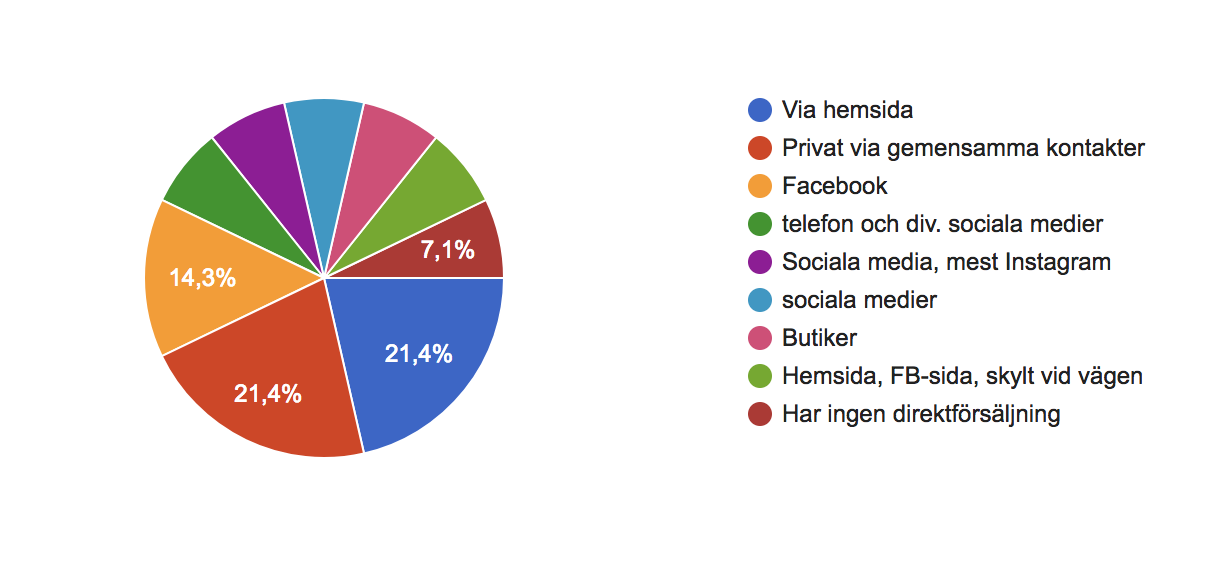
\includegraphics[scale=0.6]{4.png}
\end{figure}

\begin{figure}[H]
	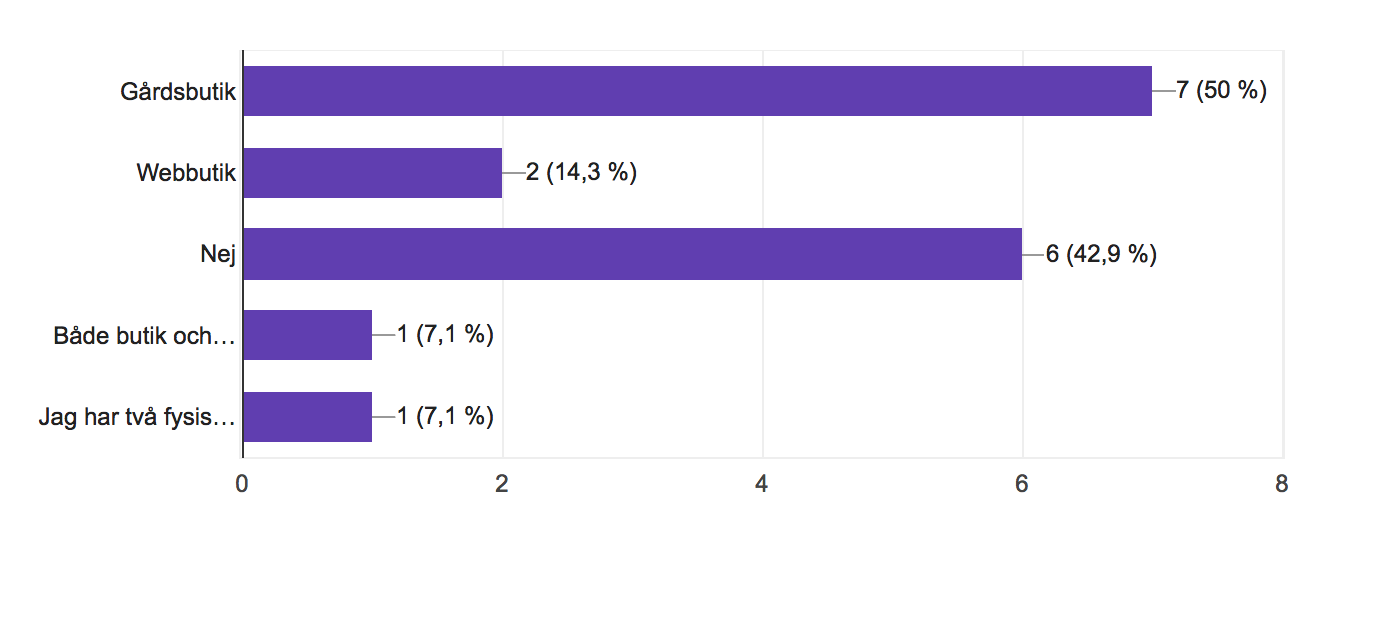
\includegraphics[scale=0.6]{5.png}
\end{figure}

\begin{figure}[H]
	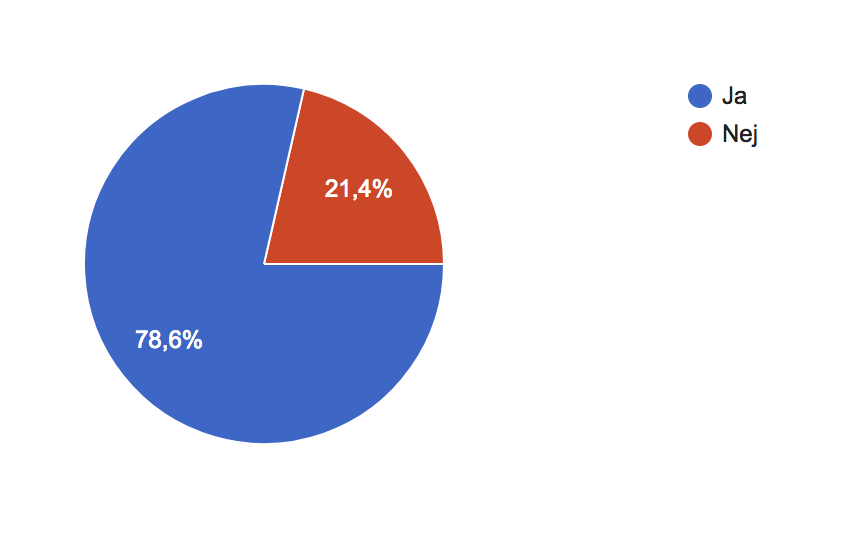
\includegraphics[scale=0.6]{6.png}
\end{figure}

\begin{figure}[H]
	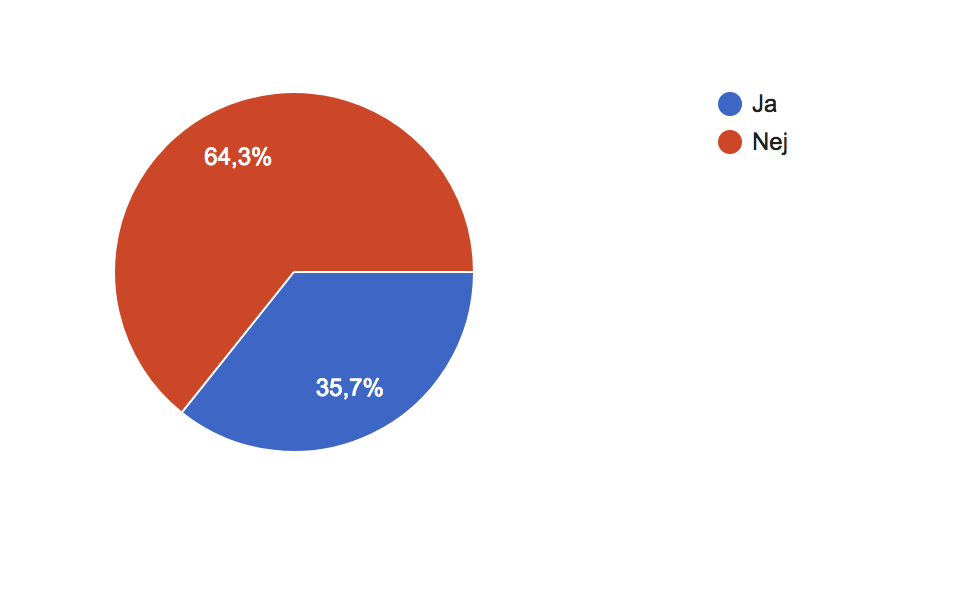
\includegraphics[scale=0.6]{7.png}
\end{figure}

\begin{figure}[H]
	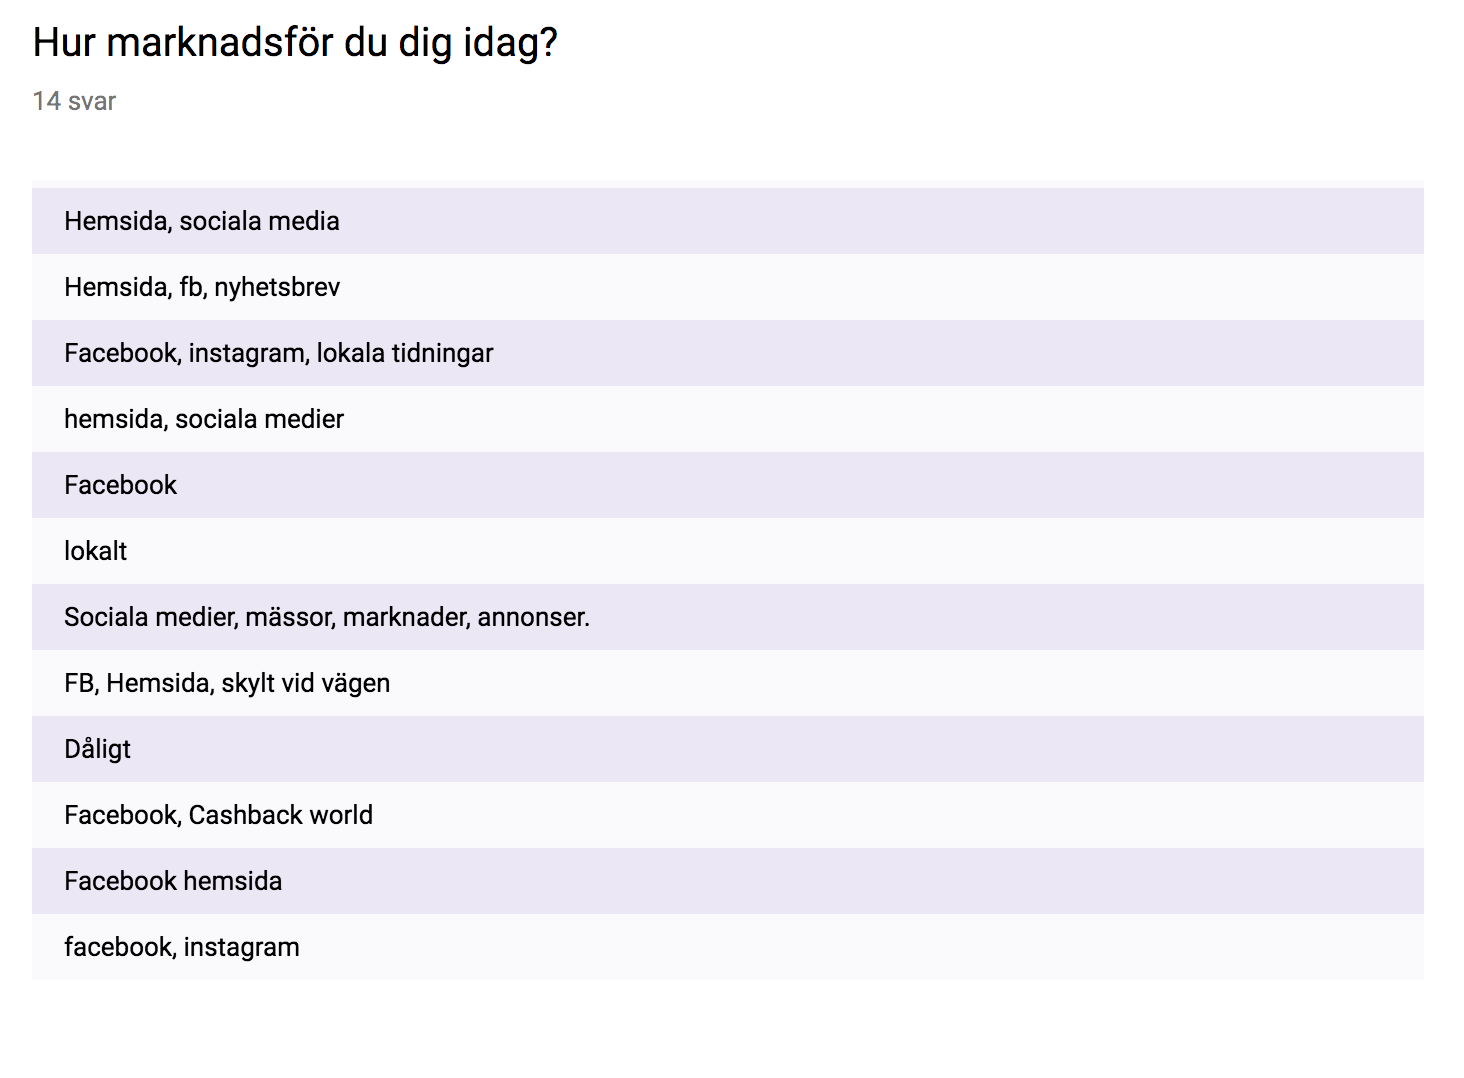
\includegraphics[scale=0.6]{8.png}
\end{figure}

\begin{figure}[H]
	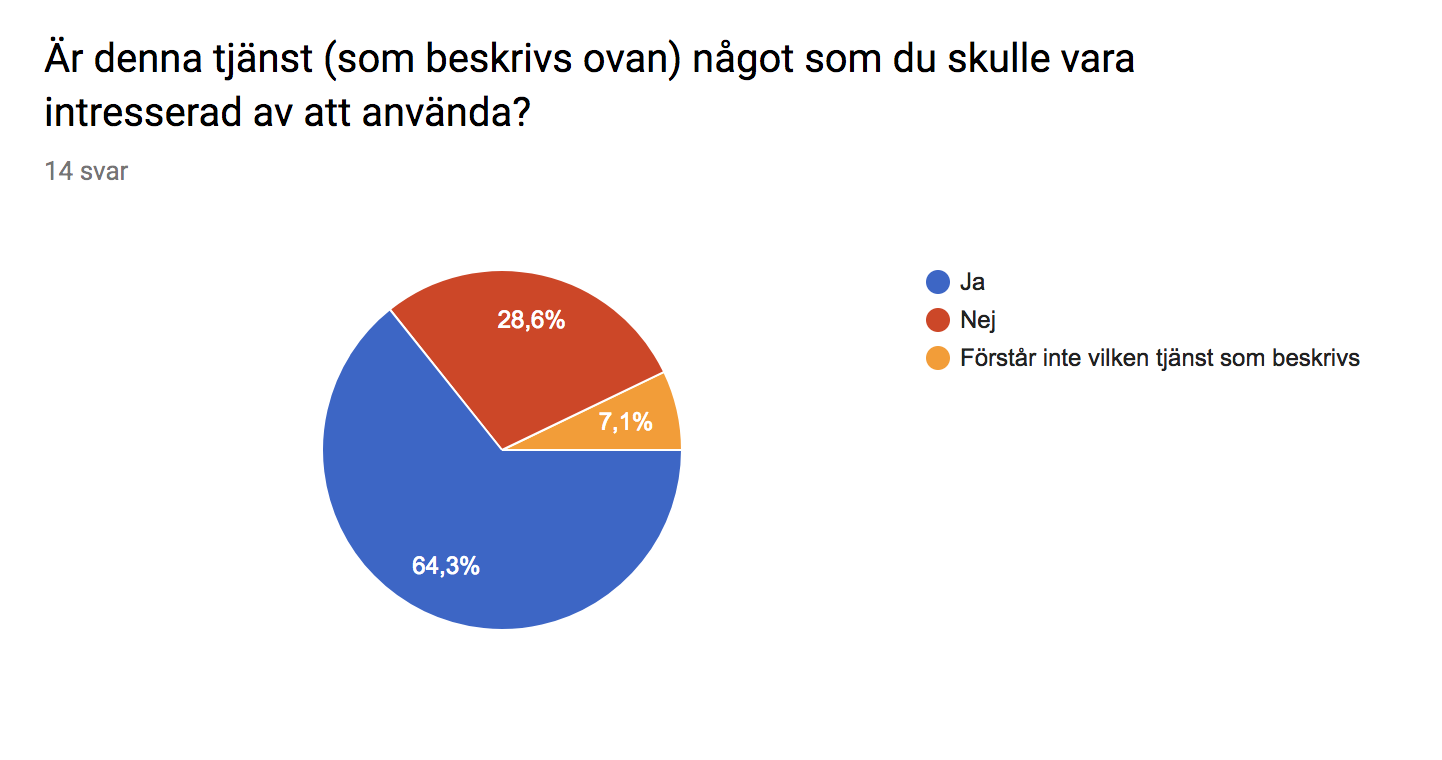
\includegraphics[scale=0.6]{9.png}
\end{figure}

\begin{figure}[H]
	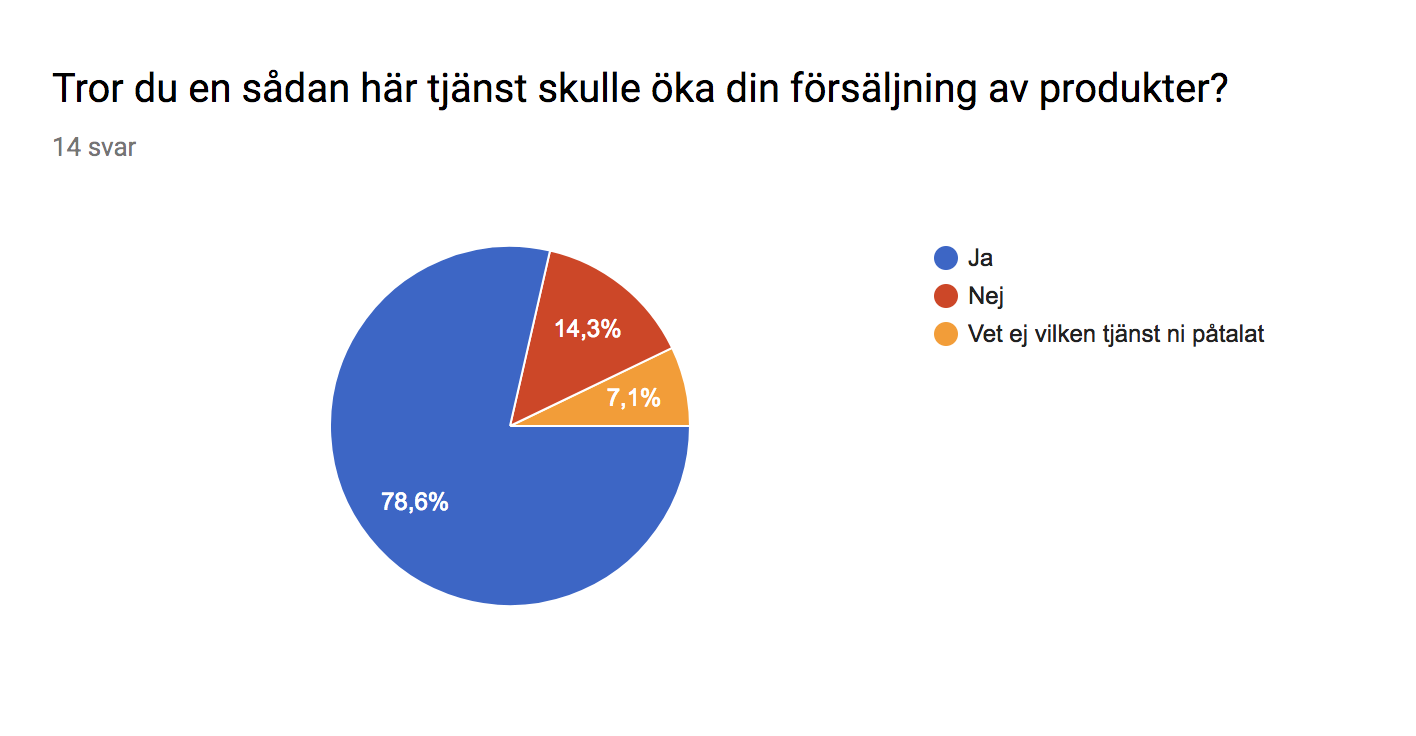
\includegraphics[scale=0.6]{10.png}
\end{figure}

\begin{figure}[H]
	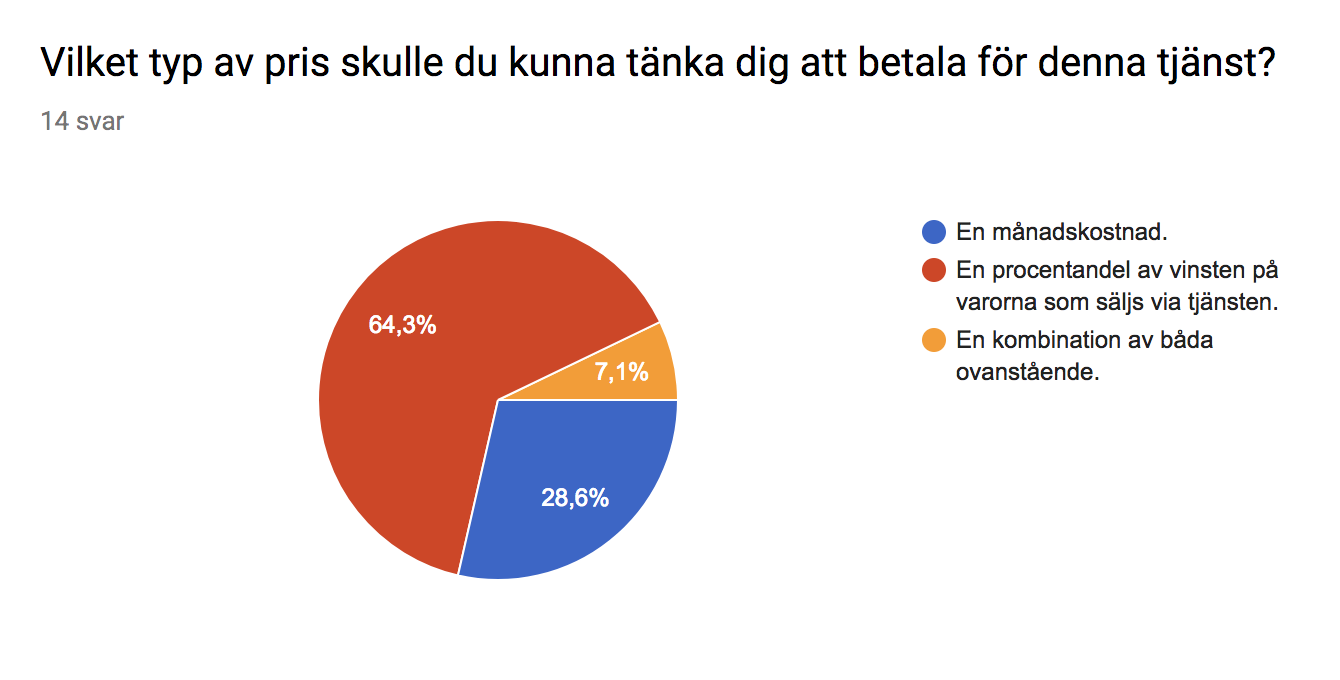
\includegraphics[scale=0.6]{11.png}
\end{figure}

\begin{figure}[H]
	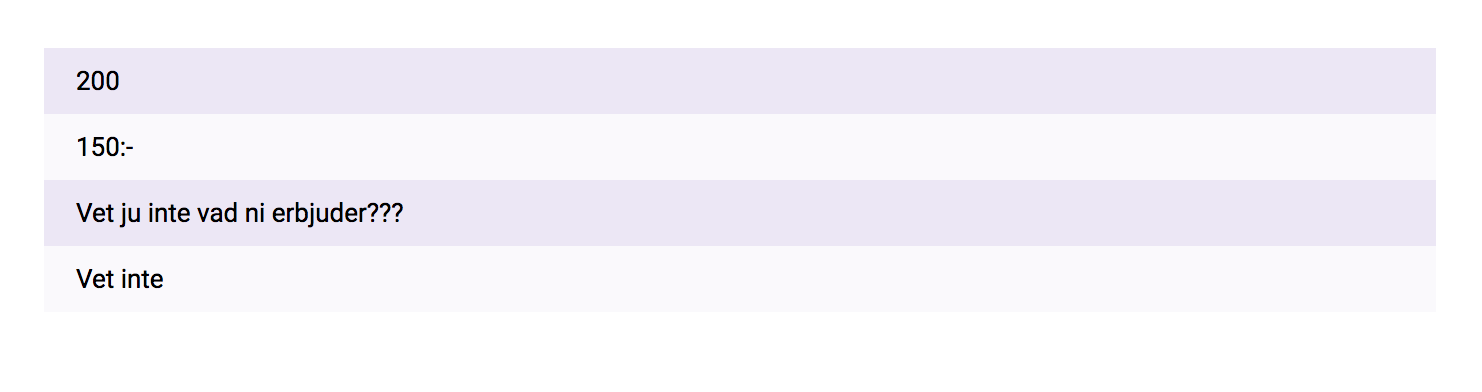
\includegraphics[scale=0.6]{12.png}
\end{figure}

\begin{figure}[H]
	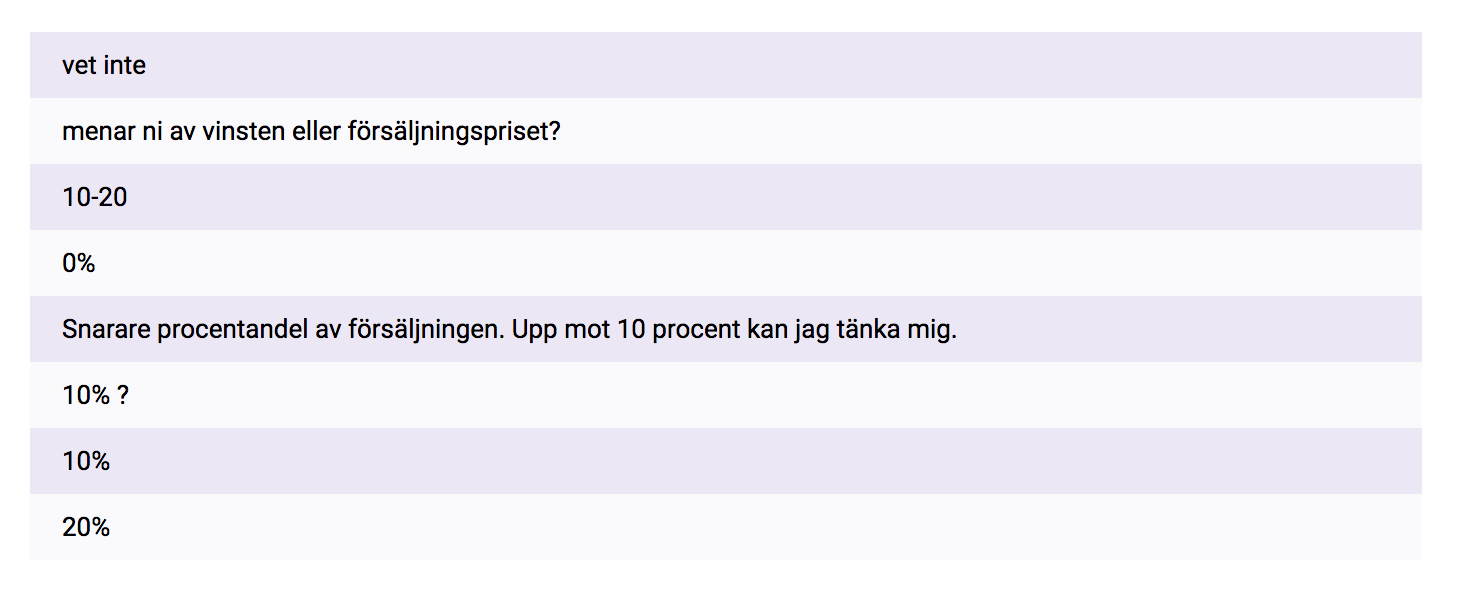
\includegraphics[scale=0.6]{13.png}
\end{figure}

\begin{figure}[H]
	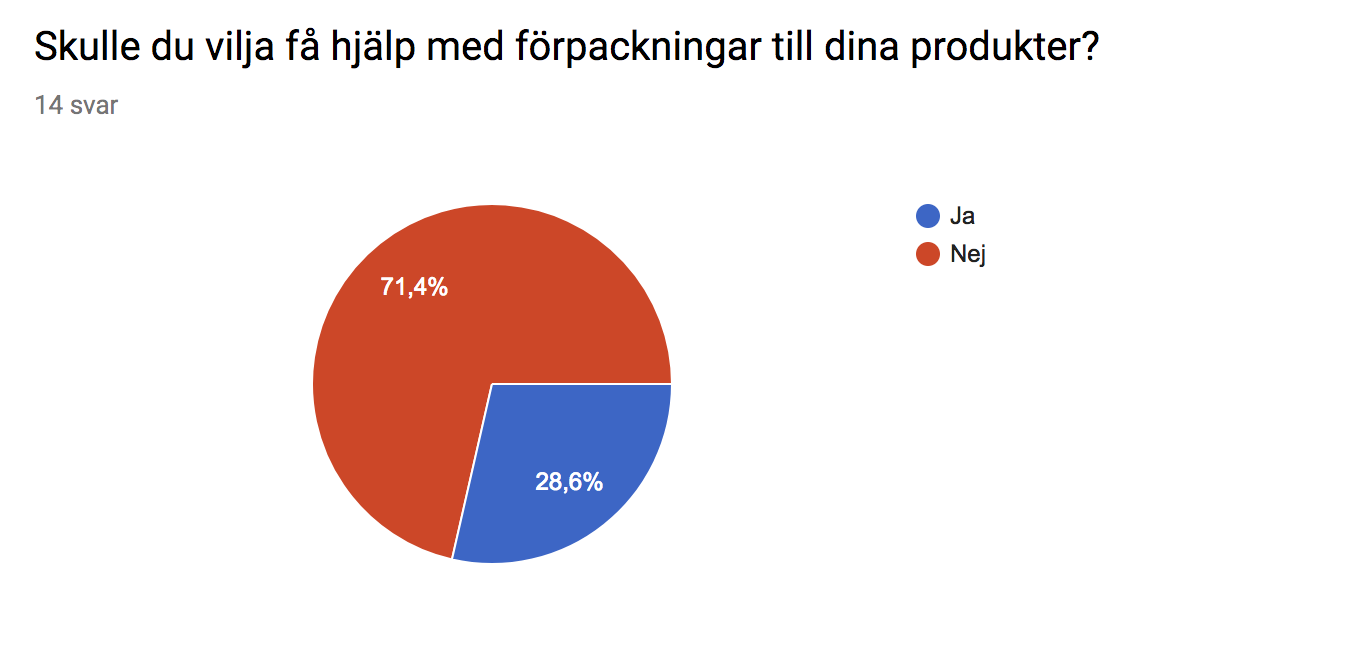
\includegraphics[scale=0.6]{14.png}
\end{figure}


\end{document}